\chapter{Introduction}\label{chap:introduction}
%
The cart pendulum is a common system subjected to different control tasks. It is interesting because it is relatively simple while still being an underactuated, and nonlinear system. This makes it an ideal platform for investigating and comparing control strategies. The system is effectively controlled by a force on the side of the cart and it being underactuated there is no direct control on the pendulum attached to the cart.\\
This project is two-part. Both parts deals with the cart pendulum system, however, while the first part considers a real system setup with frictions, the second part uses the same parameters but without any friction.\\
\textbf{First part} contains a description of the supplied system setup and a model derivation first using Newton's method then using the energy method. Finally a sliding mode controller is designed and implemented, both in simulation and in the real system, to stabilize the system in zero.\\
\textbf{Second part} contains a method for planning trajectories in the phase plane. This enables the possibility of solving tasks where the system is required to move in the nonlinear phase plane. The task solved in this project is seen in \autoref{fig:systemTask}, where the pendulum must follow a planned trajectory to avoid the two obstacles.
%
\begin{figure}[H]
  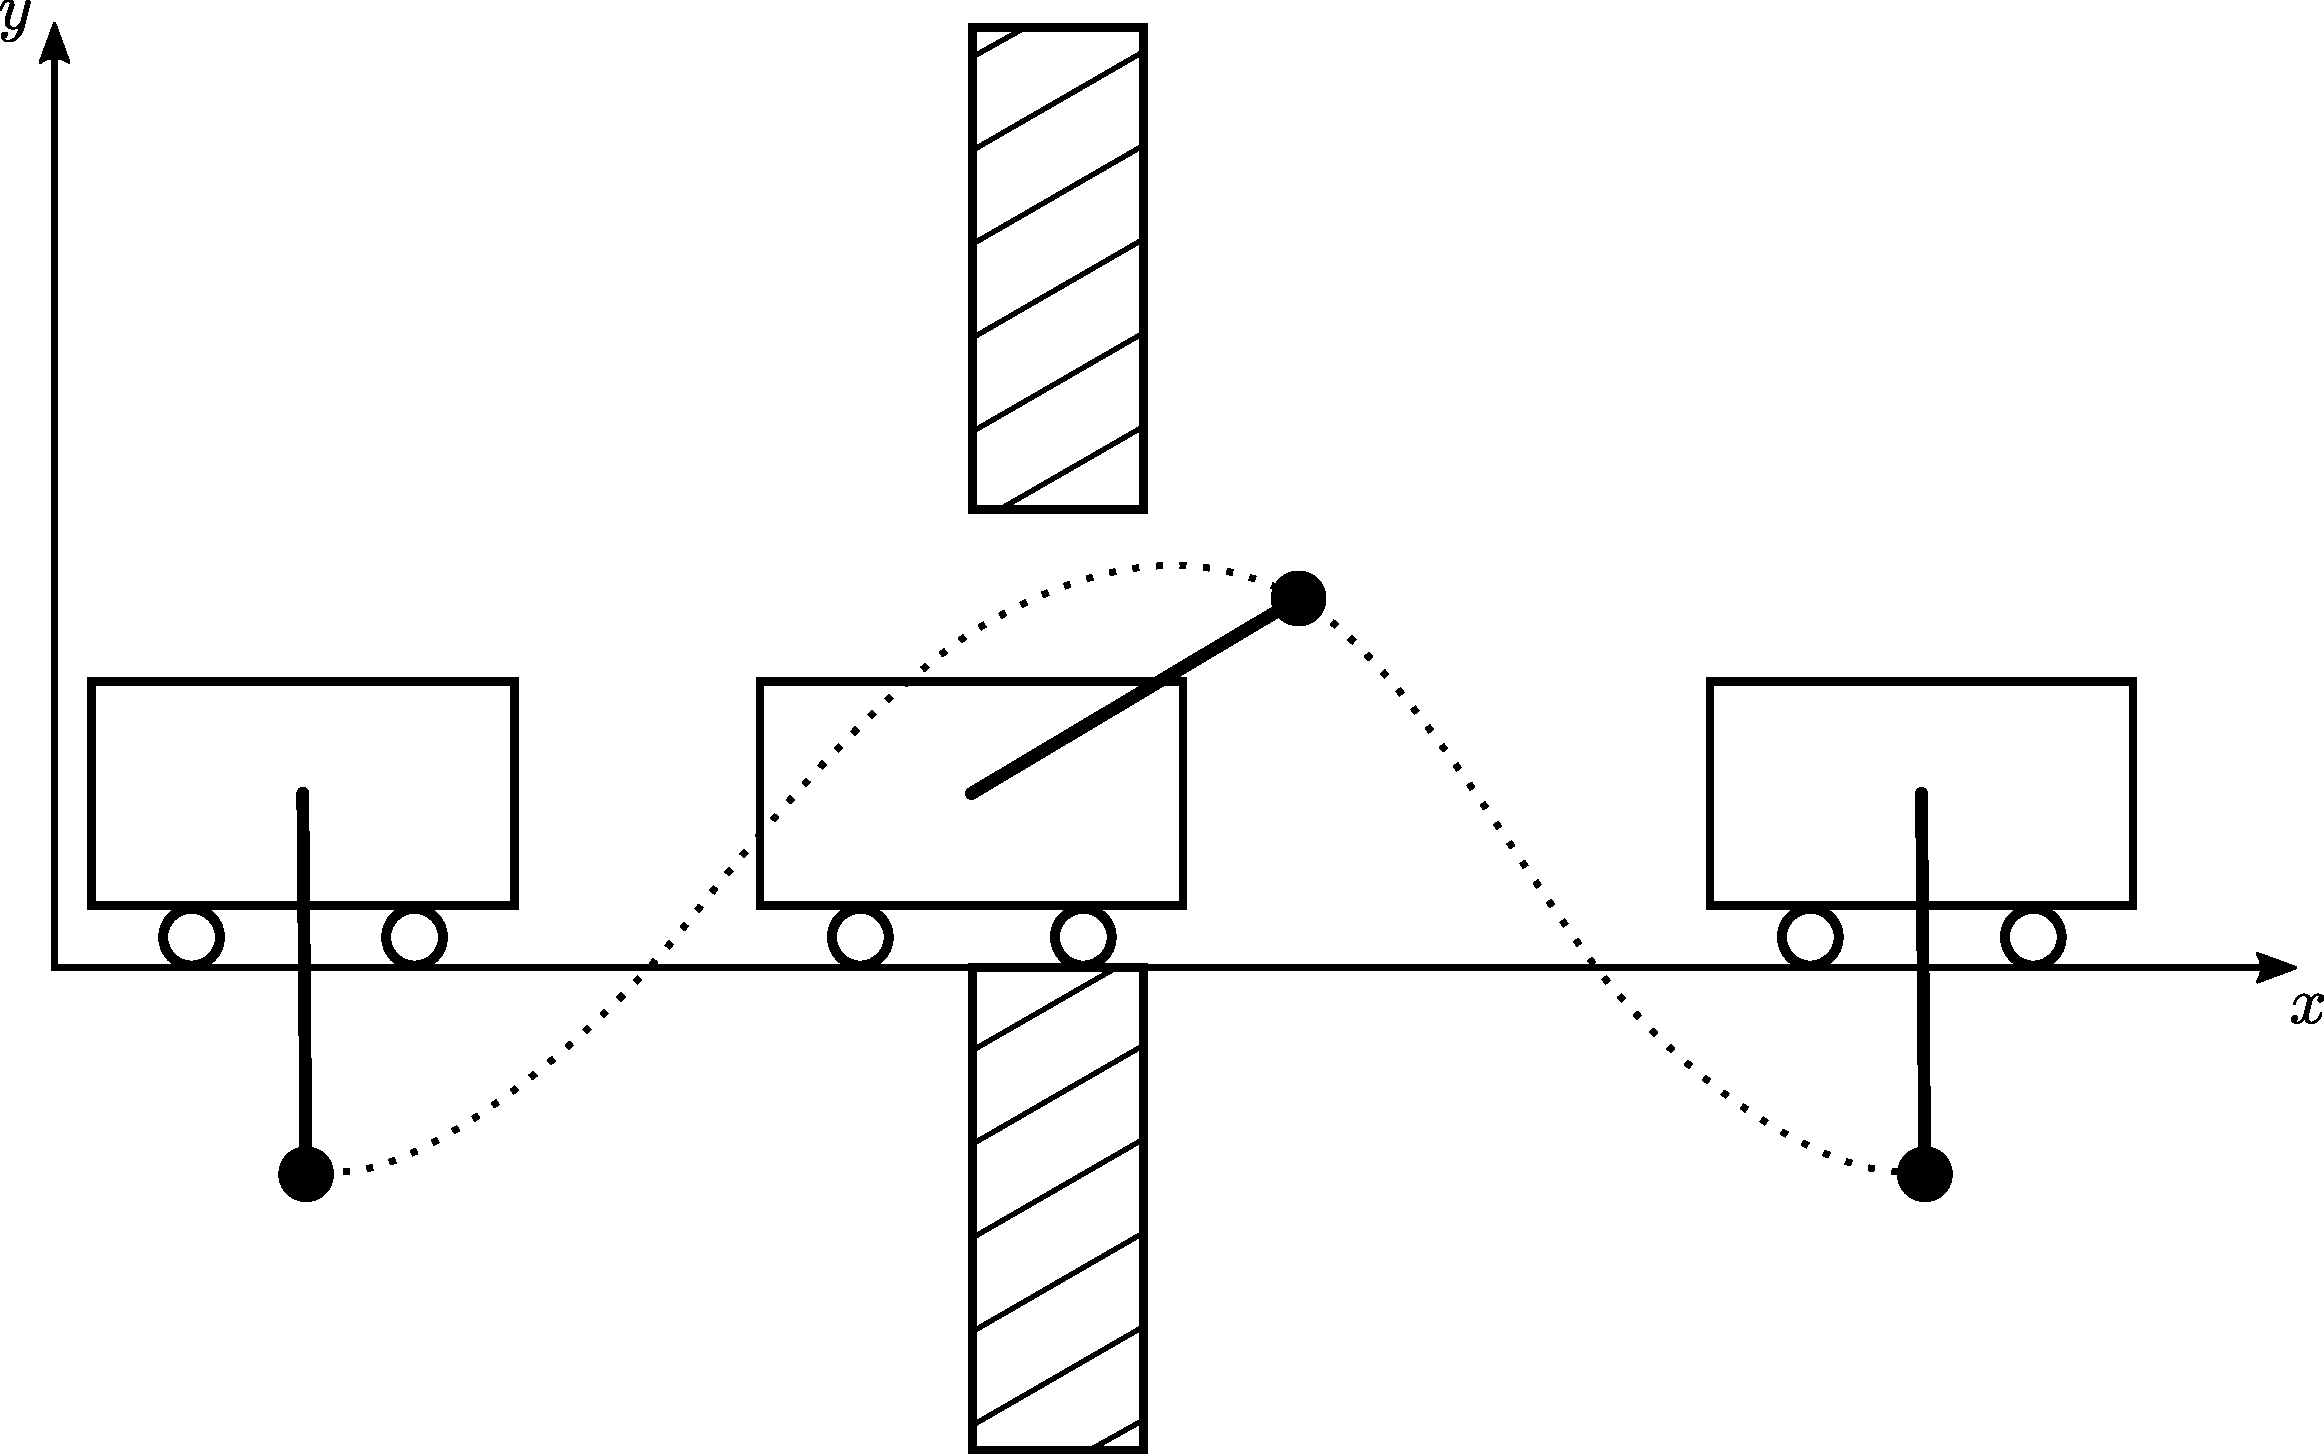
\includegraphics[width=.6\textwidth]{figures/systemTask}
  \caption{The task to be performed in part two. The trajectory here is not realistic, and only shown to illustrate the goal; avoiding the obstacles along the entire trajectory.}
  \label{fig:systemTask}
\end{figure}
%
As mentioned, friction is removed for the second part. This is both to reduce complexity but also because the system setup is too short for the large movements required to complete the task. The control for this part is therefore run in simulation and an animation is developed to visualize the result.

%The system in \autoref{fig:system}, is the well-known cart pendulum system. The system can only be controlled by a the force shown directly on the cart in the horisontal direction. So the system is underactuated, and nonlinear.

%\begin{figure}[H]
%  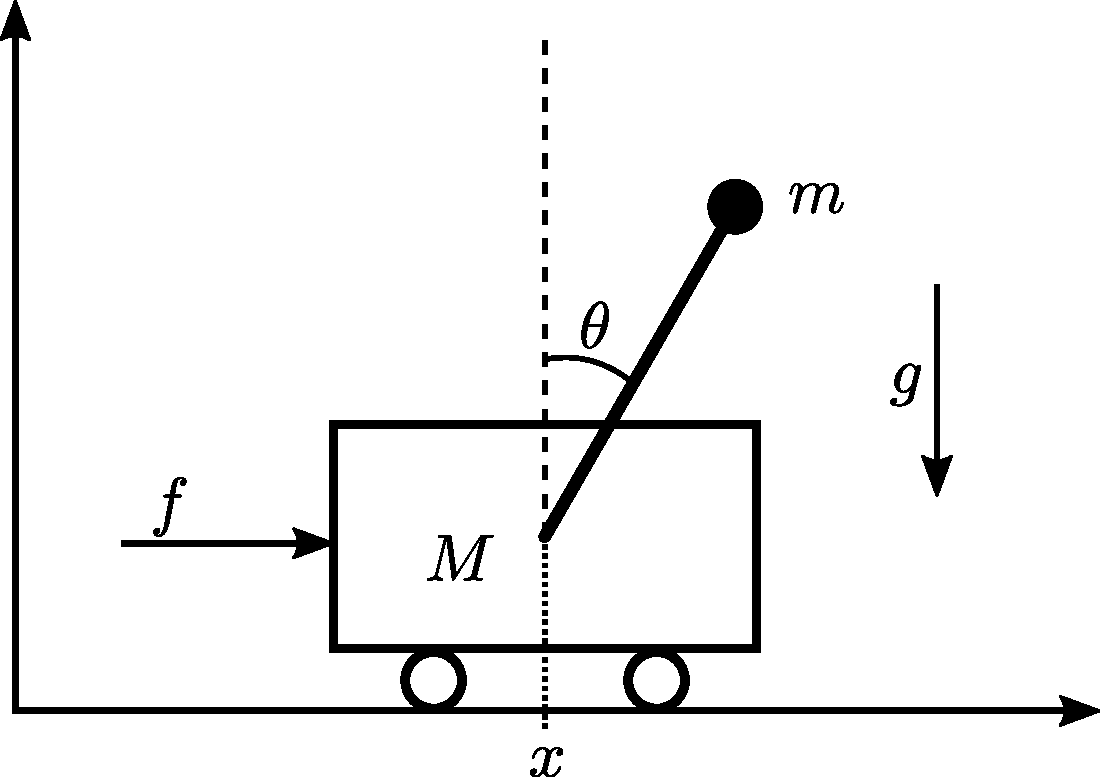
\includegraphics[width=.4\textwidth]{figures/system}
%  \caption{The cart pendulum system with generalized coordinates, $x$ and $\theta$, where $x$ is the center position of the cart, $\theta$ is the angle of the pendulum, $m$ is the point mass of the pendulum, $M$ is the mass of the cart, g is the gravitational acceleration and f is the force of actuation.}
%  \label{fig:system}
%\end{figure}

